% --- ETUDE DE CAS ---
\newpage
\section*{Étude de cas~: Burnout}
\addcontentsline{toc}{section}{Étude de cas~: Burnout}

\section*{AAV}
\addcontentsline{toc}{section}{AAV}
\begin{itemize}
	\item [1] Décrire .NET Core et .NET Framework et leur rôle dans .Net
	\item [1] Décrire les architectures .NET (Core et Framework)
	\item [2] Expliquer les évolutions entre .NET Core et .NET Framework
	\item [2] Expliquer les notions de CoreCLR et CLR (architecture, composants, processus d'exécution, gestion automatique de la mémoire)
	\item [2] Expliquer les notions d'assemblage pour .NET Core et .NET Framework (déploiement, GAC)
	\item [1] Connaître les principaux outils supportant la chaine d'intégration continue
	\item [1] Connaître les principes généraux de la conteneurisation et ses avantages en terme de déploiement de solutions
	\item [1] Connaître les environnements et outils Docker
	\item [3] Pratiquer l'installation et la configuration de Git
	\item [3] Relier Visual Studio à un dépôt Git
	\item [3] Illustrer les principes généraux de gestion de versions pour un fichier et Appliquer les commandes Git associées
\end{itemize}

\newpage

\subsection*{Mots clés}
\phantomsection
\addcontentsline{toc}{subsection}{Mots clés}
\begin{itemize}
	\item POO
	\item Génie logiciel
	\item Modularité
	\item Build
	\item Versionning
	\item Tests unitaires
	\item Classes
	\item Objets
	\item Déploiement
	\item Application
	\item Régression
	\item Fichier source
\end{itemize}

\subsection*{Contexte}
\phantomsection
\addcontentsline{toc}{subsection}{Contexte}
\noindent L'entreprise 2F Roaming s'est étendu de 2 développeurs à une équipe de 20 personnes, tout en conservant des méthodes de travail obsolètes. Ce manque de structuration a engendré des difficultés majeures, des problèmes de qualité, de productivité et de gestions des versions. Face à ces défis, Mathilde a été mandatée pour moderniser les pratiques de développement et instaurer une culture DevOps au sein de l'équipe.

\subsection*{Problématique}
\phantomsection
\addcontentsline{toc}{subsection}{Problématique}
\noindent Comment améliorer les pratiques de développement logiciel chez 2F Roaming pour garantir la qualité, la productivité et la gestion efficace des versions dans un environnement en croissance rapide ?

\subsection*{Contraintes}
\phantomsection
\addcontentsline{toc}{subsection}{Contraintes}
\begin{itemize}
	\item POO
	\item Automatisation des tests
	\item IDE compatible avec POO
	\item Multi-plateforme
\end{itemize}

\subsection*{Généralisation}
\phantomsection
\addcontentsline{toc}{subsection}{Généralisation}
\begin{itemize}
	\item POO
	\item Génie logiciel
\end{itemize}

\subsection*{Livrables}
\phantomsection
\addcontentsline{toc}{subsection}{Livrables}
\begin{itemize}
	\item Plan d'amélioration
	\begin{itemize}
		\item Environnement de développement
		\item Gestion de versions
		\item Colaboration
		\item Tests automatisés
	\end{itemize}
\end{itemize}

\subsection*{Pistes de solutions}
\phantomsection
\addcontentsline{toc}{subsection}{Pistes de solutions}
\begin{itemize}
	\item Se renseigner sur les solutions de gestion de versions (Git, SVN)
	\item Etudier les test automatisés
	\item Mettre en place un environnement de développement standardisé
	\item Former l'équipe aux nouvelles pratiques
\end{itemize}

\subsection*{Plan d'actions}
\phantomsection
\addcontentsline{toc}{subsection}{Plan d'actions}
\begin{itemize}
	\item Analyse des besoins et des pratiques actuelles
	\item Recherche et sélection des outils adaptés
	\begin{itemize}
		\item Gestion de versions (Git)
		\item Intégration continue (Jenkins, GitLab CI)
		\item Tests automatisés (JUnit, Selenium)
		\item Environnement de développement (IDE, conteneurs)
	\end{itemize}
	\item Mise en place de l'environnement de développement
	\item Documentation des nouvelles pratiques
\end{itemize}

\newpage
\section*{Démarche~: Burnout}
\addcontentsline{toc}{section}{Démarche~: Burnout}


\subsection*{Définition~: Mots clés}
\phantomsection
\addcontentsline{toc}{subsection}{Définition: Mots clés}

\noindent \textbf{POO}:
\noindent La Programmation Orientée Objet (\textbf{POO}) est un paradigme de programmation qui utilise des "objets" pour représenter des données et des méthodes. Un \textbf{objet} est une \textbf{instance} d'une \textbf{classe}, qui peut être considérée comme un modèle ou un plan définissant les attributs et les comportements de l'objet.

\vspace{0.5cm}

\noindent \textbf{Les classes} : Une classe est une structure qui définit les attributs et les méthodes que ses objets peuvent posséder. Elle sert de plan pour créer des objets.
\begin{minted}{csharp}
public class Voiture
{
	private string marque;
	private string modele;

	public string Marque 
	{ 
		get { return marque; } 
		set { marque = value; } 
	}
	public string Modele 
	{ 
		get { return modele; } 
		set { modele = value; } 
	}

	public Voiture(string marque, string modele)
	{
		this.marque = marque;
		this.modele = modele;
	}

	public void Demarrer()
	{
		Console.WriteLine($"{Marque} {Modele} démarre.");
	}
}

/* Exemple de classe "Voiture" avec des attributs privés et des
propriétés publiques */
\end{minted}

\newpage

\noindent \textbf{Les objets} : Un objet est une instance d'une classe. Il contient des données et des méthodes définies par la classe.

\vspace{0.5cm}

\noindent \textbf{Les attributs} : En Python, les attributs d’un objet englobent à la fois les variables (ou propriétés) et les méthodes. Tout ce qui est associé à une instance ou à la classe elle-même est considéré comme un attribut.

\vspace{0.5cm}

\noindent \textbf{Les méthodes} : Les méthodes sont des fonctions définies à l'intérieur d'une classe. Elles décrivent les comportements des objets de cette classe.

\vspace{0.5cm}

\noindent \textbf{L'encapsulation} : L'encapsulation est le principe de restreindre l'accès direct à certaines données d'un objet et de contrôler cet accès via des méthodes. Cela protège les données internes de l'objet contre les modifications non autorisées. Pour cela, on utilise un underscore \_ devant le nom de l'attribut.

\vspace{0.5cm}

\noindent \textbf{L'héritage} : L'héritage permet à une classe de dériver d'une autre classe, en héritant de ses attributs et méthodes. Cela favorise la réutilisation du code et la création de hiérarchies de classes.

\vspace{0.5cm}

\noindent \textbf{Polymorphisme} : Le polymorphisme permet à des objets de classes différentes d'être traités comme des objets de la même classe via des interfaces communes. Cela permet d'utiliser des méthodes dans une interface commune sans connaître les détails des classes spécifiques.

\vspace{0.5cm}

\noindent \textbf{Abstraction} :L'abstraction consiste à créer des classes abstraites qui définissent des méthodes communes sans implémenter leur logique. Ce sont les classes dérivées qui implémentent ces méthodes.

\vspace{0.5cm}

\noindent A quoi sert la POO~?

\begin{itemize}
	\item \textbf{Réutilisation du code} : Grâce à l'héritage, le code peut être réutilisé, ce qui réduit la duplication et facilite la maintenance.
	\item \textbf{Modularité} : La POO permet de diviser un programme en morceaux indépendants (classes et objets), rendant le code plus facile à comprendre et à maintenir.
    \item \textbf{Extensibilité} : Les programmes orientés objet sont plus faciles à étendre. De nouvelles fonctionnalités peuvent être ajoutées en créant de nouvelles classes ou en modifiant les classes existantes sans affecter le reste du programme.
    \item \textbf{Encapsulation} : L'encapsulation protège les données et assure une manipulation cohérente et sécurisée des attributs de l'objet.
\end{itemize}

\newpage

\noindent \textbf{Génie logiciel}:
\noindent Est appelé \textbf{génie logiciel} l'application des principes de l'\textbf{ingénierie} (traitant habituellement des \textbf{systèmes physiques}) à la \textbf{conception}, au \textbf{développement}, au \textbf{test}, au \textbf{déploiement} et à la \textbf{gestion de logiciels}.

\noindent Cette discipline applique au \textbf{développement logiciel} l'approche \textbf{structurée} et \textbf{hiérarchisée} de la programmation utilisée par l'ingénierie, dans le but d'améliorer la \textbf{qualité}, les \textbf{délais} et le \textbf{budget}, tout en assurant des \textbf{tests ordonnés} et la \textbf{certification des ingénieurs}.

\vspace{0.5cm}

\noindent \textbf{API}: Une API (application programming interface ou « interface de programmation d’application ») est une interface logicielle qui permet de « connecter » un logiciel ou un service à un autre logiciel ou service afin d’échanger des données et des fonctionnalités. Les API offrent de nombreuses possibilités, comme la portabilité des données, la mise en place de campagnes de courriels publicitaires, des programmes d’affiliation, l’intégration de fonctionnalités d’un site sur un autre ou l’open data. Elles peuvent être gratuites ou payantes.

\vspace{0.5cm}

\noindent \textbf{Modularité}: C'est l'étape de transformation. On prend les fichiers sources (la recette) et on les compile/prépare pour qu'ils deviennent un fichier exécutable par l'ordinateur. C'est le moment où la recette devient un plat prêt à être servi.

\vspace{0.5cm}

\noindent \textbf{Build}: C'est l'étape de transformation. On prend les fichiers sources (la recette) et on les compile/prépare pour qu'ils deviennent un fichier exécutable par l'ordinateur. C'est le moment où la recette devient un plat prêt à être servi.

\vspace{0.5cm}

\noindent \textbf{Versionning}: C'est la machine à remonter le temps du code. Via des outils comme Git, on enregistre chaque modification. Si on fait une erreur catastrophique aujourd'hui, on peut revenir exactement à l'état du code d'hier à 14h02. C'est aussi ce qui permet à 100 développeurs de travailler sur le même fichier sans s'écraser les uns les autres.

\vspace{0.5cm}

\noindent \textbf{Tests unitaires}: Ce sont des petits gardiens automatisés. Un test unitaire vérifie une seule petite fonctionnalité (une "unité") de manière isolée.

\noindent Exemple : On écrit un test pour vérifier que la fonction "Addition" renvoie bien 4 quand on lui donne 2+2. Si demain elle renvoie 5, le test passe au rouge.

\vspace{0.5cm}

\noindent \textbf{Déploiement}: C'est l'étape où l'on envoie le code (après le build et les tests) sur les serveurs réels pour que les utilisateurs puissent y accéder. Passer de "ça marche sur mon ordi" à "c'est disponible sur Internet".

\vspace{0.5cm}

\noindent \textbf{Application}: C'est le résultat final, l'ensemble complet et fini. C'est l'outil avec lequel l'utilisateur interagit (ton application Instagram, ton logiciel de compta, etc.). C'est la somme de tous les modules, objets et builds mentionnés plus haut.

\newpage

\noindent \textbf{Régression}: Il y a "régression" quand on répare un bug à gauche, mais que cela en crée un nouveau à droite (ou qu'un ancien bug réapparaît). C'est pour éviter cela qu'on fait des tests : pour s'assurer qu'ajouter une fonctionnalité ne fait pas reculer la qualité globale.

\vspace{0.5cm}

\noindent \textbf{Fichier source}: C'est le document de base écrit par le développeur. Imagine une recette de cuisine écrite sur papier : c'est du texte lisible par l'humain (en Python, Java, C++, etc.), mais ce n'est pas encore le plat final. C'est la matière première.

\subsection*{L'écosystème .NET : Framework vs Core}
\phantomsection
\addcontentsline{toc}{subsection}{L'écosystème .NET : Framework vs Core}
\noindent Aujourd'hui, on parle simplement de .NET (5, 6, 7, 8) qui est la fusion et l'évolution de tout ce qui suit.

\begin{center}
	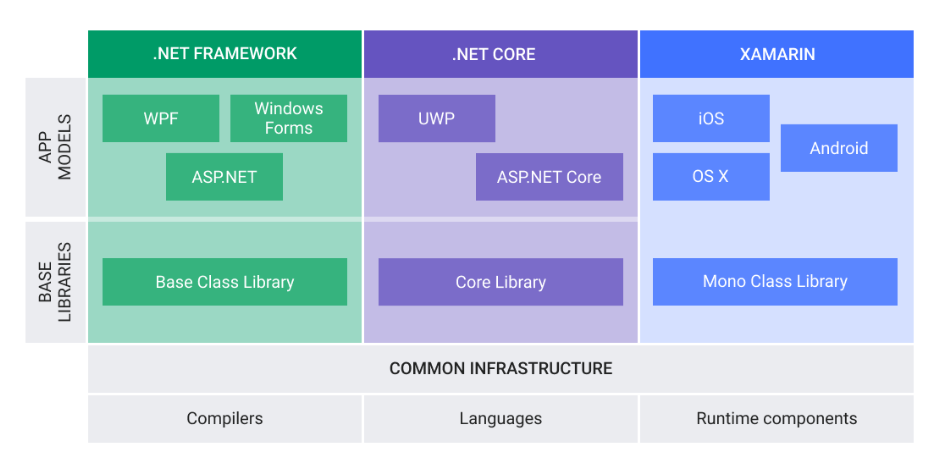
\includegraphics[width=\textwidth]{contents/img/NET.png}
\end{center}

\begin{itemize}
	\item \textbf{.NET Framework (L'ancêtre)} : Conçu exclusivement pour Windows. C'est le moteur historique pour les applications de bureau (WPF, WinForms) et le Web ancien (ASP.NET WebForms).
	\item \textbf{.NET Core (Le renouveau)} : Une version réécrite de zéro, cross-platform (Windows, Linux, macOS). Il est beaucoup plus rapide, léger et conçu pour le Cloud et les micro-services.
	\item \textbf{Leur rôle} : Fournir une bibliothèque de code (Base Class Library) et un environnement d'exécution pour que ton code tourne de la même manière partout.
\end{itemize}

\newpage

\noindent Le passage du Framework au Core a marqué trois ruptures :

\begin{itemize}
	\item \textbf{Performance} : .NET Core est drastiquement plus rapide.
	\item \textbf{Modularité} : Contrairement au Framework qui est un bloc monolithique installé sur Windows, .NET Core est distribué via des paquets NuGet. On n'embarque que ce dont on a besoin.
	\item \textbf{Open Source} : .NET Core est totalement ouvert à la communauté, contrairement au Framework original.
\end{itemize}

\vspace{0.5cm}

\subsection*{L'architecture interne : CLR et CoreCLR}
\phantomsection
\addcontentsline{toc}{subsection}{L'architecture interne : CLR et CoreCLR}
\noindent Le CLR (Common Language Runtime) est le cœur du moteur. C'est lui qui "exécute" le code.

\begin{itemize}
	\item \textbf{Composants \& Processus d'exécution}
	\begin{itemize}
		\item 1. Ton code C\# est compilé en CIL (Common Intermediate Language).
		\item 2. Le CLR prend ce CIL et le transforme en code machine (0 et 1).
		\item 3. La compilation JIT (Just-In-Time).
	\end{itemize}
	\item \textbf{Gestion de la mémoire (Garbage Collector)} : Tu n'as pas à détruire les objets manuellement. Le Garbage Collector (GC) surveille les objets qui ne sont plus utilisés et libère la mémoire automatiquement pour éviter les fuites.
\end{itemize}

\vspace{0.5cm}

\noindent \textbf{Les Assemblages (Assembly)}
\noindent Un assemblage est le résultat du build (souvent un .dll ou un .exe).
\begin{itemize}
	\item \textbf{Sur .NET Framework} : On utilisait souvent le GAC (Global Assembly Cache), un dossier centralisé dans Windows où toutes les applications piochaient leurs librairies. C'était parfois le "DLL Hell" (conflits de versions).
	\item \textbf{Sur .NET Core} : Le GAC n'existe plus. Chaque application emporte ses propres dépendances avec elle (déploiement autonome), garantissant qu'elle fonctionnera partout sans polluer le système.
\end{itemize}

\newpage
    
\subsection*{Conteneurisation et Docker}
\phantomsection
\addcontentsline{toc}{subsection}{Conteneurisation et Docker}
\noindent La conteneurisation (avec Docker) consiste à emballer ton application avec tout ce dont elle a besoin (OS minimal, runtime .NET, librairies) dans une "boîte" isolée appelée Conteneur.

\begin{itemize}
	\item \textbf{Avantage} : "Ça marche sur mon ordi, donc ça marchera sur le serveur". On élimine les problèmes d'environnement.
	\item \textbf{Outils} : \textbf{Docker Desktop} (pour développer), Docker Hub (pour stocker les images) et les fichiers Dockerfile (la recette de fabrication de l'image).
\end{itemize}

\vspace{0.5cm}

\subsection*{Intégration Continue (CI) et Git}
\phantomsection
\addcontentsline{toc}{subsection}{Intégration Continue (CI) et Git}
\noindent \textbf{La chaîne d'intégration (CI)}
\noindent C'est l'automatisation. Dès que tu pousses du code sur Git, des outils s'activent pour vérifier que tout est OK :

\begin{itemize}
	\item \textbf{Azure DevOps / GitHub Actions / GitLab CI} : Les chefs d'orchestre.
	\item \textbf{SonarQube} : Analyse la qualité du code.
	\item \textbf{Tests automatiques} : Exécution des tests unitaires définis plus haut.
\end{itemize}

\noindent \textbf{Maîtriser Git (Commandes clés)}
\noindent Pour utiliser Git avec Visual Studio, on relie généralement l'IDE à un dépôt distant (GitHub/Azure Repos) via l'onglet "Git Changes".

\vspace{0.5cm}

\begin{table}[ht]
    \centering
    \begin{tabularx}{\textwidth}{l l X}
        \toprule
        \textbf{Action} & \textbf{Commande Git} & \textbf{Explication} \\
        \midrule
        Initialiser & \texttt{git init} & Prépare le dossier pour le versionning. \\
        \addlinespace
        Staging & \texttt{git add .} & Met les changements dans le "panier" avant de valider. \\
        \addlinespace
        Valider & \texttt{git commit -m "msg"} & Enregistre une version (un point de sauvegarde). \\
        \addlinespace
        Envoyer & \texttt{git push} & Envoie tes sauvegardes sur le serveur distant. \\
        \addlinespace
        Récupérer & \texttt{git pull} & Récupère le travail des collègues. \\
        \bottomrule
    \end{tabularx}
	\caption{Commandes de base Git}
\end{table}
    

\newpage

\section*{Corbeille d'Excercice - Git}
\addcontentsline{toc}{section}{Corbeille d'Excercice - Git}

\subsection*{Initialisation d'un dépôt Git}
\phantomsection
\addcontentsline{toc}{subsection}{Initialisation d'un dépôt Git}
\noindent \textbf{Objectif} : Initialiser un dépôt Git local et effectuer les premières opérations de base.4

\begin{enumerate}
	\item Ouvrez votre terminal ou invite de commandes.
	\item Naviguez jusqu'au répertoire où vous souhaitez créer un nouveau projet.
	\item Exécutez la commande suivante pour initialiser un dépôt Git :
	\begin{minted}{bash}
git init MonProjet
	\end{minted}
	\item Accédez au répertoire du projet :
	\begin{minted}{bash}
cd MonProjet
	\end{minted}
	\item Créez un fichier README.md avec une description de votre projet.
	\item Ajoutez le fichier au suivi Git :
	\begin{minted}{bash}
git add README.md
	\end{minted}
	\item Effectuez votre premier commit :
	\begin{minted}{bash}
git commit -m "Premier commit : ajout du README"
	\end{minted}
\end{enumerate}

\subsection*{Gestion des branches}
\phantomsection
\addcontentsline{toc}{subsection}{Gestion des branches}
\noindent \textbf{Objectif} : Créer et gérer des branches dans un dépôt Git.

\begin{enumerate}
	\item Depuis le répertoire de votre projet, créez une nouvelle branche nommée "develop" :
	\begin{minted}{bash}
git branch develop
	\end{minted}
	\item Basculez sur la branche "develop" :
	\begin{minted}{bash}
git checkout develop
	\end{minted}
	\item Modifiez le fichier README.md en ajoutant une nouvelle section.
	\item Ajoutez et validez vos modifications :
	\begin{minted}{bash}
git add README.md
git commit -m "Ajout d'une section dans le README sur la branche develop"
	\end{minted}
	\item Revenez à la branche principale (main) :
	\begin{minted}{bash}
git checkout main
	\end{minted}
	\newpage
	\item Fusionnez les modifications de la branche "develop" dans "main" :
	\begin{minted}{bash}
git merge develop
	\end{minted}
	\item Vérifiez l'état de votre dépôt après la fusion :
	\begin{minted}{bash}
git status
	\end{minted}
\end{enumerate}

\subsection*{Résolution de conflits}
\phantomsection
\addcontentsline{toc}{subsection}{Résolution de conflits}
\noindent \textbf{Objectif} : Simuler et résoudre un conflit de fusion dans Git.

\begin{enumerate}
	\item Sur la branche "main", modifiez le fichier README.md en ajoutant une ligne différente de celle que vous avez ajoutée sur la branche "develop".
	\item Ajoutez et validez vos modifications sur la branche "main" :
	\begin{minted}{bash}
git add README.md
git commit -m "Modification du README sur la branche main"
	\end{minted}
	\item Basculez à nouveau sur la branche "develop" :
	\begin{minted}{bash}
git checkout develop
	\end{minted}
	\item Tentez de fusionner la branche "main" dans "develop" :
	\begin{minted}{bash}
git merge main
	\end{minted}
	\item Git signalera un conflit. Ouvrez le fichier README.md et résolvez le conflit en choisissant quelle modification conserver.
	\item Après avoir résolu le conflit, ajoutez le fichier modifié :
	\begin{minted}{bash}
git add README.md
	\end{minted}
	\item Finalisez la fusion en effectuant un commit :
	\begin{minted}{bash}
git commit -m "Résolution du conflit entre main et develop"
	\end{minted}
\end{enumerate}

\subsection*{Utilisation d'un dépôt distant}
\phantomsection
\addcontentsline{toc}{subsection}{Utilisation d'un dépôt distant}
\noindent \textbf{Objectif} : Connecter un dépôt Git local à un dépôt distant et effectuer des opérations de push et pull.

\begin{enumerate}
	\item Créez un nouveau dépôt sur GitHub (ou une autre plateforme Git distante) sans initialiser de README, .gitignore ou licence.
	\item Dans votre terminal, ajoutez le dépôt distant à votre dépôt local :
	\begin{minted}{bash}
git remote add origin

git push -u origin main
	\end{minted}
	\newpage
	\item Poussez vos commits locaux vers le dépôt distant :
	\begin{minted}{bash}
git push origin main
	\end{minted}
	\item Pour simuler une modification distante, allez sur GitHub et modifiez le fichier README.md directement dans l'interface web, puis validez les modifications.
	\item Revenez à votre terminal et récupérez les modifications distantes :
	\begin{minted}{bash}
git pull origin main
	\end{minted}
\end{enumerate}

\subsection*{Revert et Reset}
\phantomsection
\addcontentsline{toc}{subsection}{Revert et Reset}
\noindent \textbf{Objectif} : Apprendre à annuler des modifications avec les commandes revert et reset.

\begin{enumerate}
	\item Effectuez une modification dans le fichier README.md et validez-la :
	\begin{minted}{bash}
git add README.md
git commit -m "Modification temporaire du README"
	\end{minted}
	\item Utilisez la commande revert pour annuler ce commit tout en conservant l'historique :
	\begin{minted}{bash}
git revert HEAD
	\end{minted}
	\item Maintenant, effectuez une autre modification dans le fichier README.md et validez-la :
	\begin{minted}{bash}
git add README.md
git commit -m "Autre modification temporaire du README"
	\end{minted}
	\item Utilisez la commande reset pour annuler ce commit et revenir à l'état précédent (attention, cela supprimera le commit de l'historique) :
	\begin{minted}{bash}
git reset --hard HEAD~1
	\end{minted}
\end{enumerate}

\subsection*{Visualiser l'historique des commits}
\phantomsection
\addcontentsline{toc}{subsection}{Visualiser l'historique des commits}
\noindent \textbf{Objectif} : Utiliser les commandes Git pour visualiser l'historique des commits.

\begin{enumerate}
	\item Utilisez la commande suivante pour afficher l'historique des commits avec des détails :
	\begin{minted}{bash}
git log --oneline --graph --decorate --all
	\end{minted}
	\item Explorez les options de la commande git log pour personnaliser l'affichage selon vos besoins.
	\begin{minted}{bash}
git log --since="2 weeks ago" --author="VotreNom"		
	\end{minted}
	\item Essayez d'afficher les différences entre deux commits spécifiques en utilisant la commande git diff.
	\begin{minted}{bash}
git diff <commit1> <commit2>
	\end{minted}
	\item Utilisez la commande git show pour afficher les détails d'un commit particulier.
	\begin{minted}{bash}
git show <commit-hash>
	\end{minted}
	\item Expérimentez avec d'autres options de git log, comme --since, --author, ou --stat, pour filtrer et afficher l'historique des commits de différentes manières.
\end{enumerate}

\subsection*{Stashing des modifications}
\phantomsection
\addcontentsline{toc}{subsection}{Stashing des modifications}
\noindent \textbf{Objectif} : Apprendre à utiliser la fonctionnalité de stashing pour sauvegarder temporairement des modifications non validées.

\begin{enumerate}
	\item Effectuez des modifications dans le fichier README.md sans les valider.
	\item Utilisez la commande suivante pour sauvegarder temporairement vos modifications :
	\begin{minted}{bash}
git stash
	\end{minted}
	\item Pour récupérer vos modifications mises de côté, utilisez la commande suivante :
	\begin{minted}{bash}
git stash pop
	\end{minted}
\end{enumerate}

\subsection*{Création et utilisation de tags}
\phantomsection
\addcontentsline{toc}{subsection}{Création et utilisation de tags}
\noindent \textbf{Objectif} : Apprendre à créer et utiliser des tags dans Git pour marquer des versions spécifiques du code.

\begin{enumerate}
	\item Créez un tag annoté pour marquer une version spécifique de votre projet :
	\begin{minted}{bash}
git tag -a v1.0 -m "Version 1.0"
	\end{minted}
	\item Listez tous les tags existants dans votre dépôt :
	\begin{minted}{bash}
git tag
	\end{minted}
	\item Poussez le tag vers le dépôt distant :
	\begin{minted}{bash}
git push origin v1.0
	\end{minted}
	\item Pour revenir à une version spécifique marquée par un tag, utilisez la commande checkout :
	\begin{minted}{bash}
git checkout v1.0
	\end{minted}
\end{enumerate}

\newpage

\subsection*{Configuration de Git}
\phantomsection
\addcontentsline{toc}{subsection}{Configuration de Git}
\noindent \textbf{Objectif} : Configurer Git avec vos informations utilisateur et préférences.
\begin{enumerate}
	\item Configurez votre nom d'utilisateur global :
	\begin{minted}{bash}
git config --global user.name "VotreNom"
	\end{minted}
	\item Configurez votre adresse e-mail globale :
	\begin{minted}{bash}
git config --global user.email "VotreEmail@example.com"
	\end{minted}
\end{enumerate}

\subsection*{Ignorer des fichiers avec .gitignore}
\phantomsection
\addcontentsline{toc}{subsection}{Ignorer des fichiers avec .gitignore}
\noindent \textbf{Objectif} : Apprendre à utiliser un fichier .gitignore pour exclure certains fichiers ou répertoires du suivi Git.

\begin{enumerate}
	\item Créez un fichier nommé .gitignore à la racine de votre projet.
	\item Ajoutez des règles pour ignorer certains fichiers ou répertoires. Par exemple, pour ignorer tous les fichiers .log et le répertoire temp/ :
	\begin{minted}{text}
*.log
temp/
	\end{minted}
	\item Enregistrez le fichier .gitignore et ajoutez-le au suivi Git :
	\begin{minted}{bash}
git add .gitignore
git commit -m "Ajout du fichier .gitignore"
	\end{minted}
\end{enumerate}

\subsection*{Collaboration avec des Pull Requests}
\phantomsection
\addcontentsline{toc}{subsection}{Collaboration avec des Pull Requests}
\noindent \textbf{Objectif} : Apprendre à collaborer avec des Pull Requests (PR) sur une plateforme Git distante comme GitHub.

\begin{enumerate}
	\item Forkez un dépôt existant sur GitHub pour créer une copie dans votre compte.
	\item Clonez votre fork localement :
	\begin{minted}{bash}
git clone <projet-fork-url>
	\end{minted}
	\item Créez une nouvelle branche pour vos modifications :
	\begin{minted}{bash}
git checkout -b ma-nouvelle-fonctionnalite
	\end{minted}
	\item Apportez des modifications au code, ajoutez et validez-les :
	\begin{minted}{bash}
git add .
git commit -m "Ajout d'une nouvelle fonctionnalité"
	\end{minted}
	\newpage
	\item Poussez votre branche vers votre fork sur GitHub :
	\begin{minted}{bash}
git push origin ma-nouvelle-fonctionnalite
	\end{minted}
	\item Allez sur GitHub et créez une Pull Request depuis votre branche vers la branche principale du dépôt original.
\end{enumerate}

\subsection*{Rebase vs Merge}
\phantomsection
\addcontentsline{toc}{subsection}{Rebase vs Merge}
\noindent \textbf{Objectif} : Comprendre la différence entre rebase et merge dans Git.

\begin{enumerate}
	\item Créez une nouvelle branche "feature" à partir de "main" et apportez des modifications.
	\item Basculez sur la branche "main" et apportez des modifications différentes.
	\item Revenez à la branche "feature" et essayez de fusionner "main" en utilisant merge :
	\begin{minted}{bash}
git merge main
	\end{minted}
	\item Résolvez les conflits s'il y en a, puis validez la fusion.
	\item Maintenant, revenez à la branche "feature" et essayez de réappliquer les modifications de "main" en utilisant rebase :
	\begin{minted}{bash}
git rebase main
	\end{minted}
	\item Résolvez les conflits s'il y en a, puis continuez le rebase :
	\begin{minted}{bash}
git rebase --continue
	\end{minted}
\end{enumerate}

\subsection*{Nettoyage du dépôt avec git gc}
\phantomsection
\addcontentsline{toc}{subsection}{Nettoyage du dépôt avec git gc}
\noindent \textbf{Objectif} : Apprendre à utiliser la commande git gc pour nettoyer et optimiser le dépôt Git.

\begin{enumerate}
	\item Exécutez la commande suivante pour lancer le processus de nettoyage et d'optimisation :
	\begin{minted}{bash}
git gc
	\end{minted}
	\item Observez les messages affichés pour comprendre ce qui a été nettoyé ou optimisé.
\end{enumerate}

\newpage

\subsection*{Utilisation avancée de git log}
\phantomsection
\addcontentsline{toc}{subsection}{Utilisation avancée de git log}
\noindent \textbf{Objectif} : Explorer les options avancées de la commande git log pour une meilleure visualisation de l'historique des commits.

\begin{enumerate}
	\item Utilisez la commande suivante pour afficher l'historique des commits avec des détails :
	\begin{minted}{bash}
git log --oneline --graph --decorate --all
	\end{minted}
	\item Explorez les options de la commande git log pour personnaliser l'affichage selon vos besoins.
	\begin{minted}{bash}
git log --since="2 weeks ago" --author="VotreNom"		
	\end{minted}
	\item Essayez d'afficher les différences entre deux commits spécifiques en utilisant la commande git diff.
	\begin{minted}{bash}
git diff <commit1> <commit2>
	\end{minted}
	\item Utilisez la commande git show pour afficher les détails d'un commit particulier.
	\begin{minted}{bash}
git show <commit-hash>
	\end{minted}
	\item Expérimentez avec d'autres options de git log, comme --since, --author, ou --stat, pour filtrer et afficher l'historique des commits de différentes manières.
\end{enumerate}

\subsection*{Configuration avancée de Git}
\phantomsection
\addcontentsline{toc}{subsection}{Configuration avancée de Git}
\noindent \textbf{Objectif} : Explorer les options de configuration avancée de Git.
\begin{enumerate}
	\item Configurez l'éditeur de texte par défaut pour Git (par exemple, Vim ou Nano) :
	\begin{minted}{bash}
git config --global core.editor "vim"
	\end{minted}
	\item Activez la coloration syntaxique dans le terminal pour une meilleure lisibilité :
	\begin{minted}{bash}
git config --global color.ui auto
	\end{minted}
	\item Configurez un alias pour une commande Git fréquemment utilisée (par exemple, git status) :
	\begin{minted}{bash}
git config --global alias.st status
	\end{minted}
\end{enumerate}

\newpage

\section*{Workshop}
\addcontentsline{toc}{section}{Workshop}

La programmation orientée objet (POO) consiste à définir des objets logiciels et à les faire interagir entre eux.

\subsection*{A1. Notion de classe}
\phantomsection
\addcontentsline{toc}{subsection}{A1. Notion de classe}
\noindent Une classe est un "moule" ou un plan de construction. Elle définit les caractéristiques (attributs) et les actions (méthodes) communes à un ensemble d'objets.

\vspace{0.5cm}

\begin{minted}{csharp}
public class Point 
{
    public double X; // Attribut (ou champ)
    public double Y;
}
\end{minted}

\subsection*{A2. Notion d'objets / Instances}
\phantomsection
\addcontentsline{toc}{subsection}{A2. Notion d'objets / Instances}
\noindent Un objet est une incarnation concrète d'une classe. En C\#, on utilise le mot-clé new pour créer un objet en mémoire (tas/heap).

\vspace{0.5cm}

\begin{minted}{csharp}
Point p1 = new Point(); // Instance de la classe Point
p1.X = 10.5;
\end{minted}

\subsection*{A3. Notion de visibilité}
\phantomsection
\addcontentsline{toc}{subsection}{A3. Notion de visibilité}
\noindent C\# utilise des modificateurs d'accès pour contrôler la sécurité des données :

\begin{itemize}
	\item \textbf{public} : accessible de partout.
	\item \textbf{private} : accessible uniquement à l'intérieur de la classe (par défaut).
	\item \textbf{protected} : accessible dans la classe et ses enfants (héritage).
	\item \textbf{internal} : accessible dans tout le projet (assembly).
\end{itemize}

\newpage

\subsection*{A4. Notion d'encapsulation (Propriétés)}
\phantomsection
\addcontentsline{toc}{subsection}{A4. Notion d'encapsulation (Propriétés)}
\noindent En C\#, on n'utilise presque jamais de champs publics. On utilise des Propriétés pour protéger les données.

\vspace{0.5cm}

\noindent La raison principale est le principe du \textbf{"Moindre Privilège"} :
\begin{itemize}
	\item \textbf{Encapsulation} : On protège l'objet contre une utilisation incorrecte. Si tout était public par défaut, un développeur pourrait modifier une donnée interne critique de l'extérieur, brisant ainsi la logique de la classe.
	\item \textbf{Sécurité et Maintenance} : En cachant tout par défaut, vous forcez le concepteur de la classe à réfléchir consciemment à ce qu'il veut exposer (l'interface publique). Cela permet de modifier le code interne plus tard sans casser les programmes qui utilisent votre classe.
\end{itemize}
    
    
\vspace{0.5cm}

\begin{minted}{csharp}
public class CompteBancaire
{
    private decimal _solde; // Champ privé (Backing field)

    public decimal Solde // Propriété
    {
        get { return _solde; }
        private set { 
            if (value >= 0) _solde = value; 
        }
    }
}
\end{minted}

\subsection*{A5. Les Records}
\phantomsection
\addcontentsline{toc}{subsection}{A5. Les Records}
\noindent Un \textbf{record} est une structure légère destinée à stocker des données. Contrairement aux classes, deux records sont considérés comme égaux si leurs valeurs sont identiques.

\begin{minted}{csharp}
public record Personne(string Nom, int Age); 
// Genère automatiquement constructeur, propriétés et comparaison
\end{minted}

\subsection*{A6. Types Valeur (Struct) vs Référence (Class)}
\phantomsection
\addcontentsline{toc}{subsection}{A6. Types Valeur (Struct) vs Référence (Class)}
\noindent En C\#, les types sont soit des \textbf{types valeur} (struct) soit des \textbf{types référence} (class).
\begin{itemize}
    \item \textbf{Class} : Allouée sur le \textbf{Heap} (Tas). On manipule une adresse mémoire.
    \item \textbf{Struct} : Allouée sur le \textbf{Stack} (Pile). Plus rapide pour les petits objets immuables.
\end{itemize}

\subsection*{B1. Constructeurs}
\phantomsection
\addcontentsline{toc}{subsection}{B1. Constructeurs}
\noindent Le constructeur initialise l'objet. Il porte le nom de la classe et n'a pas de type de retour.

\vspace{0.5cm}

\begin{minted}{csharp}
public class Robot
{
    public string Nom { get; set; }

    // Constructeur
    public Robot(string nom)
    {
        this.Nom = nom; // 'this' désigne l'objet actuel
    }
}
\end{minted}

\subsection*{B2. Paramètres optionnels}
\phantomsection
\addcontentsline{toc}{subsection}{B2. Paramètres optionnels}
\noindent Au lieu de créer 3 constructeurs, C\# permet de définir des valeurs par défaut.

\vspace{0.5cm}

\begin{minted}{csharp}
public Point(double x = 0, double y = 0) 
{
    X = x;
    Y = y;
}
// Appels possibles : new Point(), new Point(5), new Point(5, 10)
\end{minted}

\subsection*{B3. Références et Garbage Collector}
\phantomsection
\addcontentsline{toc}{subsection}{B3. Références et Garbage Collector}
\noindent En C\#, contrairement au C++, vous ne gérez pas la destruction des objets (pas de delete). Le Garbage Collector (ramasse-miettes) libère automatiquement la mémoire quand l'objet n'est plus utilisé.

\vspace{0.5cm}

\subsection*{B4. La directive using}
\phantomsection
\addcontentsline{toc}{subsection}{B4. La directive using}
\noindent Le Garbage Collector ne ferme pas les fichiers ou les bases de données instantanément. Le bloc \textbf{using} garantit la libération immédiate des ressources externes.

\begin{minted}{csharp}
using (var reader = new StreamReader("file.txt")) {
    // Le fichier est ouvert
} // Le fichier est fermé ici automatiquement
\end{minted}

\vspace{0.5cm}

\subsection*{C1. Membres statiques}
\phantomsection
\addcontentsline{toc}{subsection}{C1. Membres statiques}
\noindent Le mot-clé \textbf{static} signifie que le membre appartient à la classe elle-même et non à une instance particulière.

\vspace{0.5cm}

\begin{minted}{csharp}
public class Calculatrice
{
    public static double PI = 3.14159;
    
    public static double Somme(double a, double b) => a + b;
}

// Utilisation sans créer d'objet
double r = Calculatrice.PI;
\end{minted}

\subsection*{C2. LINQ (Language Integrated Query)}
\phantomsection
\addcontentsline{toc}{subsection}{C2. LINQ (Language Integrated Query)}
\noindent LINQ permet de manipuler les listes de données comme si on faisait des requêtes SQL, de façon très concise.

\begin{minted}{csharp}
var nomsLongs = listeNoms.Where(n => n.Length > 5)
                         .OrderBy(n => n)
                         .ToList();
\end{minted}

\newpage

\subsection*{D1. Héritage}
\phantomsection
\addcontentsline{toc}{subsection}{D1. Héritage}
\noindent En C\#, on utilise l'opérateur \textbf{:} pour l'héritage. Une classe ne peut hériter que d'une seule classe parente.

\vspace{0.5cm}

\begin{minted}{csharp}
public class Animal 
{
    public virtual void Crier() => Console.WriteLine("L'animal crie");
}

public class Chien : Animal 
{
    public override void Crier() => Console.WriteLine("Le chien aboie");
}
\end{minted}

\subsection*{D2. Polymorphisme (Virtual / Override)}
\phantomsection
\addcontentsline{toc}{subsection}{D2. Polymorphisme (Virtual / Override)}
\noindent Pour qu'une méthode puisse être redéfinie, elle doit être marquée \textbf{virtual} dans le parent. L'enfant utilise \textbf{override}.

\vspace{0.5cm}

\begin{minted}{csharp}
Animal monAnimal = new Chien();
monAnimal.Crier(); // Affiche "Le chien aboie" (Liaison tardive)
\end{minted}

\subsection*{D3. Classes Abstraites}
\phantomsection
\addcontentsline{toc}{subsection}{D3. Classes Abstraites}
\noindent Une classe abstract ne peut pas être instanciée. Elle sert de base à d'autres classes.

\vspace{0.5cm}

\begin{minted}{csharp}
public abstract class Forme
{
    public abstract double CalculerAire(); // Pas de corps de fonction
}
\end{minted}

\newpage

\subsection*{D4. Les Interfaces}
\phantomsection
\addcontentsline{toc}{subsection}{D4. Les Interfaces}
\noindent Une interface est un contrat. Elle définit "ce que l'objet sait faire" sans dire "comment il le fait". Une classe peut implémenter plusieurs interfaces.

\vspace{0.5cm}

\begin{minted}{csharp}
public interface IVolant
{
    void Voler();
}

public class Avion : IVolant
{
    public void Voler() { /* Code pour décoller */ }
}
\end{minted}

\subsection*{E1. Async / Await}
\phantomsection
\addcontentsline{toc}{subsection}{E1. Async / Await}
\noindent Pour éviter de figer l'interface utilisateur ou bloquer un serveur, on utilise des tâches asynchrones. Le mot-clé \textbf{await} suspend l'exécution sans bloquer le thread en attendant la fin d'une opération (ex: réseau).

\begin{minted}{csharp}
public async Task<string> GetDataAsync() {
    var result = await _httpClient.GetStringAsync("https://api.com");
    return result;
}
\end{minted}

\newpage

\section*{Analyse et résolution : Burnout}
\addcontentsline{toc}{section}{Analyse et résolution : Burnout}

L'entreprise 2F Roaming a connu une croissance rapide, passant de 2 à 20 dévelop-peurs, sans adapter ses méthodes de travail. Ce manque de structuration a entraîné des problèmes de qualité logicielle, de productivité et de gestion des versions. Pour répondre à cette problématique, il est nécessaire d'adopter une démarche structurée et progressive, centrée sur l'amélioration continue et l'intégration de pratiques modernes du génie logiciel.

\noindent \textbf{Résolution proposée~:}

\begin{itemize}
	\item \textbf{Mise en place d'un système de gestion de versions moderne (Git)}~: Permettre un suivi précis des modifications, faciliter la collaboration et garantir la traçabilité du code.
	\item \textbf{Adoption de la Programmation Orientée Objet (POO)}~: Structurer le code pour le rendre plus modulaire, maintenable et évolutif.
	\item \textbf{Automatisation des tests}~: Intégrer des tests unitaires et d'intégration pour assurer la qualité du logiciel à chaque évolution.
	\item \textbf{Standardisation de l'environnement de développement}~: Définir des outils et des configurations partagés (IDE, extensions, règles de codage) pour homogénéiser les pratiques.
	\item \textbf{Formation et accompagnement de l'équipe}~: Organiser des sessions de formation sur les nouveaux outils et méthodes, et instaurer une culture DevOps favorisant la communication et l'amélioration continue.
	\item \textbf{Mise en place de l'intégration continue (CI)}~: Automatiser les processus de build, de test et de déploiement pour accélérer les livraisons et réduire les erreurs humaines.
\end{itemize}

Cette démarche permettra à 2F Roaming d'améliorer la qualité de ses livrables, d'accroître la productivité de ses équipes et de mieux gérer la croissance de son effectif.



\subsection*{Conclusion}
\phantomsection
\addcontentsline{toc}{subsection}{Conclusion}

La modernisation des pratiques de développement chez 2F Roaming est indispensable pour accompagner la croissance de l'entreprise. En adoptant des outils adaptés (gestion de versions, automatisation des tests, CI), en structurant le code (POO) et en formant les équipes, l'entreprise pourra garantir la qualité, la productivité et la pérennité de ses projets logiciels. L'implication de tous les membres et le soutien de la direction seront les clés du succès de cette transformation.

\newpage

\section*{Capitalisation}
\addcontentsline{toc}{section}{Capitalisation}

\begin{center}
\setlength{\tabcolsep}{10pt}

\begin{tabular}{|p{0.30\textwidth}|p{0.45\textwidth}|m{0.08\textwidth}|}
\hline
\textbf{AAV} & \textbf{Commentaire} & \textbf{Statut} \\ \hline

Décrire .NET Core et .NET Framework et leur rôle dans .Net &
Les différences, rôles et évolutions sont expliqués, avec schéma et exemples. &
{\color{green!60!black}Acquis} \\ \hline

Décrire les architectures .NET &
L'architecture interne (CLR, CoreCLR, composants) est détaillée, distinctions claires. &
{\color{green!60!black}Acquis} \\ \hline

Expliquer les évolutions entre .NET Core et .NET Framework &
Les ruptures (performance, modularité, open source) sont bien identifiées et justifiées. &
{\color{green!60!black}Acquis} \\ \hline

Expliquer les notions de CoreCLR et CLR &
Explications précises sur le CLR/CoreCLR, compilation, JIT, Garbage Collector. &
{\color{green!60!black}Acquis} \\ \hline

Expliquer les notions d'assemblage pour .NET Core et .NET Framework &
Assemblages, GAC, déploiement autonome bien expliqués, différences mises en avant. &
{\color{green!60!black}Acquis} \\ \hline

Connaître les principaux outils supportant la chaine d'intégration continue &
Outils CI (Azure DevOps, GitHub Actions, GitLab CI, SonarQube) listés et expliqués. &
{\color{green!60!black}Acquis} \\ \hline

Connaître les principes généraux de la conteneurisation et ses avantages &
Principe de conteneurisation, avantages et outils (Docker, Dockerfile) présentés clairement. &
{\color{green!60!black}Acquis} \\ \hline

Connaître les environnements et outils Docker &
Docker Desktop, Docker Hub, fichiers Dockerfile mentionnés et contextualisés. &
{\color{green!60!black}Acquis} \\ \hline

Pratiquer l'installation et la configuration de Git &
Procédure d'installation, configuration utilisateur, commandes de base détaillées. &
{\color{green!60!black}Acquis} \\ \hline

Relier Visual Studio à un dépôt Git &
Lien entre Visual Studio et Git expliqué, utilisation de l'onglet "Git Changes" abordée. &
{\color{green!60!black}Acquis} \\ \hline

Illustrer les principes généraux de gestion de versions pour un fichier et Appliquer les commandes Git associées &
Principes de versionning, commandes Git (init, add, commit, push, pull, merge, etc.) illustrés par des exemples pratiques. &
{\color{green!60!black}Acquis} \\ \hline

\end{tabular}
\end{center}

\section*{Ressources}
\addcontentsline{toc}{section}{Ressources}

\begin{itemize}
	\item \textbf{Documentation officielle de Git} : \url{https://git-scm.com/doc}
	\item \textbf{Pro Git Book} : \url{https://git-scm.com/book/en/v2}
	\item \textbf{GitHub Learning Lab} : \url{https://lab.github.com/}
	\item \textbf{POO} : \url{https://docs.microsoft.com/fr-fr/dotnet/csharp/fundamentals/object-oriented/}
	\item \textbf{C\# Guide} : \url{https://docs.microsoft.com/fr-fr/dotnet/csharp/}
	\item \textbf{LINQ} : \url{https://docs.microsoft.com/fr-fr/dotnet/csharp/programming-guide/concepts/linq/}
	\item \textbf{Async/Await} : \url{https://docs.microsoft.com/fr-fr/dotnet/csharp/programming-guide/concepts/async/}
\end{itemize}
